\documentclass[13pt,largemargins]{homework}
\author{Ornella Elena Grassi}
\title{Homework 1 }
\date{}  % Toggle commenting to test
\newcommand{\hwname}{Ornella Elena Grassi}
\newcommand{\hwemail}{s290310@studenti.polito.it}
\newcommand{\hwtype}{Homework}
\newcommand{\hwnum}{1}
\newcommand{\hwclass}{}
\newcommand{\hwlecture}{}
\newcommand{\hwsection}{}
\newcommand{\argmin}{\arg\!\min}

\usepackage{lipsum}
\usepackage{amssymb}
\usepackage[utf8]{inputenc}
\usepackage[T1]{fontenc}
\usepackage{lmodern}
\usepackage{amsfonts}
\usepackage{hyperref}
\usepackage{bbm}
\usepackage{amsmath}
\usepackage{epstopdf}
\usepackage{enumitem}
\usepackage{subcaption}
\usepackage{bbm}
\usepackage{graphicx}
\usepackage{listings}
\usepackage{mcode}

\setcounter{MaxMatrixCols}{15}

\lstset{language=Matlab,
basicstyle=\footnotesize\ttfamily,
numbers=left,
numberstyle=\tiny,
stepnumber=2,
frame=lines
}

\begin{document}
\maketitle
\begin{center}
Realizzato in collaborazione con Andrea Sanna(s222975)
\end{center}
\section %ESERCIZIO 1
\begin{enumerate}[label=(\alph*)]
\item %1a
I cammini che uniscono il nodo \textit{o} al nodo \textit{d} sono i seguenti: 
\begin{center}
	$p^{(1)}  =  o \rightarrow a \rightarrow d,$ \\
	$p^{(2)}  =  o \rightarrow b \rightarrow d,$\\
	$p^{(3)}  =  o \rightarrow a \rightarrow b \rightarrow d.$
\end{center}	

Avendo ciascun arco una capacità maggiore di uno, tutti e 3 i cammini supportano flussi unitari. Per far sì che non ci siano più flussi unitari ammissibili, è necessario che la capacità di almeno un arco di ciascuno cammino sia portata a 0 oppure, al più, ad un valore $C < 1$.\\Pertanto, sia $\varepsilon$ tale che $0 < \varepsilon< 1$, basta rimuovere una quantità pari a $2+\varepsilon$ dall'arco \(e_1\) e $1+\varepsilon$ dall'arco \(e_2\) (oppure \(e_5\)) o, equivalentemente, si può pensare di rimuovere $2+\varepsilon$ dall'arco \(e_4\) e $1+\varepsilon$ dall'arco \(e_5\). Entrambe le soluzioni apportano una riduzione minima di capacità pari a $3 + 2\varepsilon$ necessariamente distribuita come descritto. 
\item %1b
%Dal testo sappiamo che le funzioni di ritardo sono date da:\\ %%%%%%%%%%%$d_1(x)=d_5(x)=x+1, d_3(x)=1, d_2(x)=d_4(x)=5x+1$.\\
Dal teorema del \textit{Max Flow-Min Cut} il flusso massimo è pari alla somma delle capacità degli archi del taglio minimo. Nel grafo considerato i possibili tagli sono:
\begin{itemize}
\item $u_1$ associato alla partizione $\mathcal{U}_1=\{a,b,d\}$, con capacità $C^*_1=3+2=5$
\item $u_2$ associato alla partizione $\mathcal{U}_2=\{b,d\}$, \\con capacità $C^*_2=2+2+3=7$
\item $u_3$ associato alla partizione $\mathcal{U}_3=\{a,d\}$, \\con capacità $C^*_3=3+2=5$
\item $u_4$ associato alla partizione $\mathcal{U}_4=\{d\}$ \\con capacità $C^*_4=3+2=5$
\end{itemize}
Avendo perciò 3 tagli di capacità identica, pari a 5, è opportuno aggiungere le 2 unità di capacità agli archi in comune tra i 3 tagli minimi così da massimizzare il flusso. Una possibile soluzione è la seguente: 
\begin{center} 
$C'(e_1) = C(e_1)+1 = 4$ \quad $C'(e_5) = C(e_5)+1 = 3$
\end{center}

In questo modo si ottiene: 
\begin{itemize}
\item $C^*_1=4+2=6$
\item $C^*_2=2+2+4=8$
\item $C^*_3=4+2=6$
\item $C^*_4=4+2=6$\\
\end{itemize} 


\item %1c
Le funzioni di ritardo associate agli archi sono 
\begin{center}
	$d_1(x) = d_5(x) = x+1$; \quad $d_3(x) = 1$; \quad $d_2(x) = d_4(x) = 5x+1$.
\end{center}	
Essendo $z = \{z_1, z_2, z_3\}$ il vettore dei flussi sui cammini da \(o\) a \(d\)  tali che $z_1+z_2+z_3=1$, le funzioni di ritardo ad essi associate sono date da:
\begin{itemize}
\item $\Delta_1=6z_1+z_3+2$ associato al cammino $p^{(1)}: o\rightarrow a \rightarrow d$; 
\item $\Delta_2=6z_2+z_3+2$ associato a $p^{(2)}: o\rightarrow b \rightarrow d$; 
\item $\Delta_3=z_1+z_2+2z_3+3$ associato a  $p^{(3)}: o\rightarrow a\rightarrow b \rightarrow d$.\\
\end{itemize}
L'equilibrio di Wardrop è la configurazione dei flussi che corrisponde all'ottimo per l'utente, quindi se il flusso sul percorso \(i\) con \(i = 1,2,3\) è non nullo, cioè $z_i>0$, il ritardo associato al percorso \textit{i} deve soddisfare $\Delta_i\leq\Delta_j,\quad \forall j \neq i$.\\
Sia $z_1>0$ e $z_2>0$. Da queste ipotesi deve risultare necessariamente
\[\begin{cases} \Delta_1\leq \Delta_2 \Leftrightarrow 6z_1+z_3+2\leq 6z_2+z_3+2 \Leftrightarrow z_1\leq z_2\\ 
\Delta_2\leq \Delta_1 \Leftrightarrow 6z_2+z_3+2\leq 6z_1+z_3+2 \Leftrightarrow z_1\geq z_2\end{cases}\]
Da cui si ottiene $z_1=z_2$.\\\\
Si considera ora $z_3>0$, per cui deve valere 
\[\begin{cases} \Delta_3 \leq \Delta_1 \Leftrightarrow z_1+z_2+2z_3 \leq 6z_1+z_3+2 \Leftrightarrow z_3\leq 4z_1-1 \\ \Delta_1 \leq \Delta_3 \Leftrightarrow 6z_1+z_3+2 \leq z_1+z_2+2z_3\Leftrightarrow z_3\geq 4z_1-1\end{cases}\]
Quindi $z_3=4z_1-1$.

Risolvendo il sistema 
\begin{equation}
	\begin{cases}
		z_1 = z_2; \\
		z_3 =4z_1-1 \\
		z_1+z_2+z_3=1,
	\end{cases}
\end{equation}	
si ottiene la configurazione dell'equilibrio di Wardrop pari a \begin{center}
$z=(z_1, z_2, z_3)=(\frac{1}{3}, \frac{1}{3}, \frac{1}{3})$. 
\end{center} 
Il corrispondente vettore di flusso sugli archi $f^{(UO)}$ in cui ciascuna delle componenti è $f^{(UO)}_{e_i}$, ossia il flusso sull'arco $e_i$, sarà: $f^{(UO)}=(\frac{2}{3}, \frac{1}{3}, \frac{1}{3}, \frac{1}{3}, \frac{2}{3})$.\\

Il tempo totale di percorrenza (Total Travel Time) è dato dalla formula
\begin{center}
$\sum_{e \in \epsilon} C_e(f_e) =  \sum_{e \in \epsilon} d_e(f)f_e$
\end{center} e pertanto vale \[TTT=\frac{2}{3}(\frac{2}{3}+1) + \frac{1}{3}(5\frac{1}{3}+1) + 1(\frac{1}{3}) + \frac{1}{3}(5\frac{1}{3}+1) + \frac{2}{3}(\frac{2}{3}+1) =\frac{13}{3}\]. 
\item %1d
Per minimizzare il ritardo medio \(o - d\) è necessario calcolare la configurazione dei flussi tale per cui il costo totale è il minimo possibile. Occorre quindi calcolare 
\begin{center}
\[ \argmin_z z_1(z_1 + z_3 + 1 + 5z_1 + 1) + z_2(5z_2+1+z_2+z_3+1) + z_3(z_1+z_3+1+1+z_2+z_3)\] 
$s.t. \quad z_1+z_2+z_3 = 1$
\end{center} 
che equivale a risolvere 
\begin{center}
\(\argmin_z 6z_1^2 + 6z_2^2 - 3z_1 -3z_2 + 5 \)\\
$s.t. \quad z_3 = 1-z_2 - z_1$
\end{center} 
Da qui si deduce che, essendo $f''(z_1) = f''(z_2) = 12 > 0$  la funzione di costo è convessa e pertanto per trovare il minimo valore di $z_1$ e $z_2$ basta osservare dove si annulla la derivata prima. Si ottine quindi che $z_1 = z_2 = \frac{1}{4}$ e risolvendo il seguente sistema 
\begin{equation}
\begin{cases}
		z_1 = z_2 = \frac{1}{4}; \\
		z_1+z_2+z_3=1,
\end{cases}
\end{equation}

si trova $z_3 = \frac{1}{2}$ e che $z=\{\frac{1}{4}, \frac{1}{4}, \frac{1}{2}\}$.\\\\
Il corrispondente flusso sugli archi all'ottimo di sistema sarà dato da: \[f^{(SO)}=(\frac{3}{4},\frac{1}{4},\frac{1}{2}, \frac{1}{4}, \frac{3}{4})\].\\
Il ritardo medio all'ottimo di sistema è invece dato da: \[\sum_{e\in \mathcal{E}}f_e^* d(f_e^*)=\frac{1}{4}(6\frac{1}{4}+2+\frac{1}{2}+\frac{1}{4}(6\frac{1}{4}+\frac{1}{2}+2)+ \frac{1}{2}(\frac{1}{4}+\frac{1}{4}+2\frac{1}{2}+3)=\frac{17}{4}\]

\item Il prezzo dell'anarchia (PoA) è dato dal rapporto fra il ritardo medio all'equilibrio di Wardrop e il costo totale all'ottimo di sistema, quindi:
\[PoA=\frac{\frac{13}{3}}{\frac{17}{4}}=\frac{52}{51}\]

\item Per portare il \(PoA\) ad 1 bisogna far sì che il costo totale all'ottimo di sistema e quello all'equilibrio di Wardrop si eguaglino. Si deve pertanto trovare un vettore di pedaggi \(\omega \) che vada a modificare l'equilibrio di Wardrop precedente, in modo che questo coincida con l'ottimo di sistema, cioè si abbia che \(f^{(\omega^*)} = f^* \).\\ Il vettore dei pedaggi sarà perciò dato da \[ \omega_i =f_e^* d_e (f_e^*)\]
Si trova quindi che 
\begin{center}
\[\omega = (1\frac{3}{4}, 5\frac{1}{4}, 0\frac{1}{2}, 5\frac{1}{4}, 1\frac{3}{4}) = (\frac{3}{4},\frac{5}{4},0,\frac{5}{4},\frac{3}{4})\].  
\end{center}

\end{enumerate}

\newpage
 \section%ESERCIZIO 2
\begin{enumerate}[label=(\alph*)]
\item %2a
Sia $\mathcal{G}=(\mathcal{V},\mathcal{E}, W)$ il grafo assegnato. La matrice dei pesi è data da:
\[W=\begin{bmatrix}
a & 1 & 0 & 0 \\
0 & 0 & 1 & 1 \\
0 & 0 & 0 & 1 \\
1 & 1 & 0 & 0 \end{bmatrix}\]
Definendo come $w=diag(W)=(a, 0, 0, 0)$ il vettore della diagonale di W, la matrice dei pesi normalizzata P è:
\[P=D^{-1}W=\begin{bmatrix} 
\frac{a}{a+1} & \frac{1}{a+1} & 0 & 0 \\
0 & 0 & \frac{1}{2} & \frac{1}{2} \\
0 & 0 & 0 & 1\\
\frac{1}{2} & \frac{1}{2} & 0 & 0 \end{bmatrix}\]
Il Laplaciano L è:
\[L=D-W=\begin{pmatrix}
1 & -1 & 0 & 0\\
0 & 2 & -1 & -1\\
0 & 0 & 1 & -1\\
-1 & -1 & 0 & 2 \end{pmatrix}\]

\item %2b (il punto b è vuoto, non c'è una domanda)
Osserviamo che $\mathcal{G}$ è fortemente connesso e aperiodico $\forall a \geq 0$, \\infatti se $a>0$ il grafo contiene un self-loop e quindi è aperiodico, mentre se $a=0$, quindi non è più presente il self-loop, rimane aperiodico perchè contiene, ad esempio, i cicli $2\rightarrow 4 \rightarrow 1$ e $2 \rightarrow 4 \rightarrow 1 \rightarrow 2$ di lunghezza 2 e 3, che sono coprimi.
Inoltre $\mathcal{G}$ è bilanciato, cioè ogni nodo ha grado entrante pari al grado uscente.\\
\item %2c giusto perchè altrimenti è disallineato
Consideriamo la dinamica di opinione di French-De Groot sul grafo $\mathcal{G}$: $x(t+1)=Px(t)$.
Dato che $\mathcal{G}$ è fortemente connesso e aperiodico per ogni $a\geq0$, allora la dinamica converge al consenso per ogni $a\geq0$: \[\lim_{t \to \infty}x_i(t)=\pi ' x(0)= \sum_i 	\pi_i x_i(0), \forall x(0)\] dove abbiamo indicato con $\pi$ la distribuzione invariante di cent\-ra\-li\-tà, data da $\pi'=P'\pi$.\\
Dal fatto che $G$ è fortemente connesso sappiamo che $\pi_i>0\quad \forall i$. In particolare, dal fatto che $\mathcal{G}$ è bilanciato, sappiamo che la misura invariante è proporzionale al vettore dei gradi $w$. Osservando che $w\mathbbm{1}=a+1+2+1+2=a+6$, otteniamo il vettore della distribuzione invariante di centralità:
\[\pi=(\frac{a+1}{a+6}, \frac{2}{a+6},\frac{1}{a+6},\frac{2}{a+6})'.\]

\item %2d
Sia $x(0)=[-1,1,-1,1]'$ il vettore delle opinioni iniziali. Poichè il limite del profilo delle opinioni esiste per $a\geq0$ possiamo affermare che la dinamica convergerà sicuramente al consenso per $a = 0$, che possiamo calcolare come 
\begin{center}
\[\lim_{t \to \infty}x_i(t)=\sum_{i \in \mathcal{V}}\pi_ix_i(0)= \frac{1}{6}(-1)+ \frac{1}{3}(1)+\frac{1}{6}(-1)+\frac{1}{3}(1)=\frac{1}{3}.\]
\end{center}

\item  %2e
Il valore minimo di $a$ tale per cui $\lim_{t \to \infty}x_1(t) \leq 0$ con il vettore delle condizioni iniziali $x(0)$ del punto precedente si trova osservando che \[\lim_{t \to \infty}x_1(t)=\frac{1}{a+6}((-1)(a+1)+2-1+2) = \frac{2-a}{a+6}\leq0 \Leftrightarrow a\geq 2\] da cui si ottiene che il valore minimo di $a$ è $a=2$.

\item %2f 
Definiamo $f(a):=Var(\lim_{t \to \infty}x_1(t))$. Calcoliamo quindi $f(a)$ come 
\begin{multline*}f(a)= Var( \pi_1x_1(0)+\pi_2x_2(0)+\pi_3x_3(0)+\pi_4x_4(0))=\\ =\sum_{i=1}^4\pi^2_i Var(x_i(0)) = \sum_{i=1}^4\pi_i^2
=\frac{1}{(a+6)^2}((a+2)^2+4+1+4)=\end{multline*}
\[=\frac{a^2+2a+10}{(a+6)^2}\]
dove abbiamo utilizzato le proprietà della varianza, il fatto che gli $x_i(0)$ fossero variabili aleatorie indipendenti fra loro (quindi con co\-va\-rian\-za nulla) e varianza unitaria.\\
Osserviamo che tale funzione è convessa, quindi per calcolare il valore di $a$ che la minimizzi è sufficiente calcolare il valore per il quale si annulla la derivata prima:
\[f'(a)=\frac{10a-8}{(a+6)^3}=0 \Leftrightarrow a=\frac{4}{5}\]
Quindi il valore che minimizza la varianza del limite del consenso è $a=\frac{4}{5}$.
\end{enumerate}
\newpage

\section %ESERCIZIO 3

\begin{enumerate}[label=(\alph*)]
%inserire grafo ???
\item %3a
Il grafo in questione è indiretto e aciclico. Il vettore dei vertici, ordinati in ordine alfabetico, risulta essere:
\begin{gather*}
v = \{ Acciaiuoli, Albizzi, Barbadori, Bischeri, Castellani,\\
Ginori, Guadagni, Lamberteschi, Pazzi, Peruzzi,\\ Ridolfi, Salviati, Tornabuoni, Strozzi, Medici\}\\
\end{gather*}
Si procede pertanto scrivendo la matrice di adiacenza \(W\) ed il vettore dei gradi \(w_i\). 
\[W=\begin{bmatrix}
	0 & 0 & 0 & 0 & 0 & 0 & 0 & 0 & 0 & 0 & 0 & 0 & 0 & 0 & 1\\
	0 & 0 & 0 & 0 & 0 & 1 & 1 & 0 & 0 & 0 & 0 & 0 & 0 & 0 & 1\\
	0 & 0 & 0 & 0 & 1 & 0 & 0 & 0 & 0 & 0 & 0 & 0 & 0 & 0 & 1\\
	0 & 0 & 0 & 0 & 0 & 0 & 1 & 0 & 0 & 1 & 0 & 0 & 0 & 1 & 0\\
	0 & 0 & 1 & 0 & 0 & 0 & 0 & 0 & 0 & 1 & 0 & 0 & 0 & 1 & 0\\
	0 & 1 & 0 & 0 & 0 & 0 & 0 & 0 & 0 & 0 & 0 & 0 & 0 & 0 & 0\\
	0 & 1 & 0 & 1 & 0 & 0 & 0 & 1 & 0 & 0 & 0 & 0 & 1 & 0 & 1\\
	0 & 0 & 0 & 0 & 0 & 0 & 1 & 0 & 0 & 0 & 0 & 0 & 0 & 0 & 0\\
	0 & 0 & 0 & 0 & 0 & 0 & 0 & 0 & 0 & 0 & 0 & 1 & 0 & 0 & 0\\
	0 & 0 & 0 & 1 & 1 & 0 & 0 & 0 & 0 & 0 & 0 & 0 & 0 & 1 & 0\\
	0 & 0 & 0 & 0 & 0 & 0 & 0 & 0 & 0 & 0 & 0 & 0 & 0 & 1 & 1\\
	0 & 0 & 0 & 0 & 0 & 0 & 0 & 0 & 1 & 0 & 0 & 0 & 0 & 0 & 1\\
	0 & 0 & 0 & 0 & 0 & 0 & 1 & 0 & 0 & 0 & 0 & 0 & 0 & 0 & 1\\
	0 & 0 & 0 & 1 & 1 & 0 & 0 & 0 & 0 & 1 & 1 & 0 & 0 & 0 & 0\\	
	1 & 1 & 1 & 0 & 0 & 0 & 0 & 0 & 0 & 0 & 1 & 1 & 1 & 0 & 0
	\end{bmatrix}\]
	
	\begin{gather*}
	\omega_i = (1, 3, 2, 3, 3, 1, 4, 1, 1, 3, 2, 2, 2, 4, 6)\\
	\end{gather*}
La misura di centralità invariante è unica e vale: 
\begin{gather*}
	\pi_i = ( \frac{1}{38}, \frac{3}{38}, \frac{1}{19}, \frac{3}{38}, \frac{3}{38}, \frac{1}{38}, \frac{2}{19}, \frac{1}{38}, \frac{1}{38}, \frac{3}{38}, \frac{1}{19}, \frac{1}{19}, \frac{1}{19}, \frac{2}{19}, \frac{3}{19}).\\
\end{gather*}
	
	Essendo il grafo fortemente connesso e aperiodico si può concludere che la dinamica di averaging di French-De Groot converge al valore di consenso, come nell'esercizio precedente, dato dal limite: 
\[\lim_{t \to \infty}x_i(t)=\pi ' x(0)= \sum_i 	\pi_i x_i(0), \forall x(0)\] e pertanto, essendo $x(0)=[0,0,0,0,0,0,0,0,0,0,0,0,0, -1, 1]'$ il vettore delle condizioni iniziali, si ottiene che il valore finale di consenso vale: 
\[\lim_{t \to \infty}x_i(t)= (-1)\frac{2}{19}+(1)\frac{3}{19}=\frac{1}{19}\]

\item %3b 
%qui ci va il codice Matlab del secondo punto 
Si riporta ora il codice Matlab sviluppato per visualizzare l'evoluzione della dinamica di opinione dei nodi del grafo, avendo assegnato ai due nodi stubborn \(\{\text{Strozzi}, \text{Medici}\}\)  rispettivamente i valori -1, +1. 


\begin{lstlisting}
Families={'Acciaiuoli', 'Albizzi', 'Barbadori', 'Bischeri',
'Castellani', 'Ginori', 'Guadagni', 'Lamberteschi','Pazzi',
'Peruzzi', 'Ridolfi', 'Salviati', 'Tornabuoni',
'Strozzi', 'Medici'}'; 

%Matrice di adiacenza W
W = zeros(15); 

W(1,15) = 1; 					%Acciaiuoli
W(2,[6 7 15]) = 1; 				%Albizzi
W(3,[5 15]) = 1; 				%Barbadori
W(4,[7 10 14]) = 1; 			%Bischeri
W(5,[3 10 14]) = 1; 			%Castellani	
W(6,2) = 1; 					%Ginori
W(7,[2 4 8 13]) = 1; 			%Guadagni
W(8,7) = 1; 					%Lamberteschi
W(9,12) = 1; 					%Pazzi
W(10,[4 5 14]) = 1; 			%Peruzzi
W(11,[15 14]) = 1; 				%Ridolfi
W(12,[15 9]) = 1; 				%Salviati
W(13,[7 15]) = 1;        		%Tornabuoni
W(14,[4 5 10 11]) = 1;  		%Strozzi
W(15,[1 2 3 11 12 13]) = 1;     %Medici
		
%vettore delle opinioni iniziali
x = zeros(15,1); 
x(14) = -1; 
x(15) = 1; 

%calcolo matrice P
w = W*ones(15,1); 
D = diag(w); 
P = D\W; 

nR=13;            				%regular nodes
nS=2;             				%stubborn nodes
u = [-1, 1]';     				%vettore degli ingressi stubborn

Q = P(1:nR, 1:nR);   			%matrice P ristretta a RxR
E = P(1:nR, (nR+1):(nR+nS)); 	%matrice P ristretta a RxS

%INIZIALIZZAZIONI
cont = 0; 
cont_max = 50; 
epsilon = 1e-4; 				%valore di tolleranza
i = 1; 

x_new = zeros(nR,1); 			%vettore delle opinioni 
x_old = zeros(nR,1); 
X_i = zeros(nR, cont_max);      %matrice dei risultati


%CALCOLO PASSI DELLA DINAMICA
while(i && cont<cont_max)
   
    cont = cont+1; 
    
    %Salvo il vettore delle opinioni nella colonna di X_i corrispondente
    X_i(sub2ind(size(X_i),1:nR, repelem(cont, nR))) = x_new; 
    
    x_new = Q*x_old + E*u;
    
    if(x_new-x_old <= epsilon)
        i = 0; 
    else
        x_old = x_new; 
    end
    
end

%PLOT DELLE TRAIETTORIE 
X=zeros(nR+nS, cont); 			%matrice X completa
X(1:nR, :) = X_i( : , 1:cont); 
X(14, :) = u(1); 
X(15, :) = u(2);

for k = 1:(nR+nS)
    figure(2)
    hold on
    plot(1:cont, X(k,:),  'LineWidth', 1)
    grid on 
    ylim([-1.1 1.1])		
end

xlabel('Tempo', 'FontSize', 10)
ylabel('Opinioni', 'FontSize', 10)
title('Traiettorie delle opinioni dei nodi', 'FontSize', 13, 'FontWeight', 'bold')
legend(Families(1:k))


\end{lstlisting}


Di seguito si riporta il grafico così prodotto, dal quale si evince che già dopo $n\approx15$ iterazioni le opinioni dei singoli nodi si stabilizzano al loro valore finale.

\begin{figure}[h]
\centering
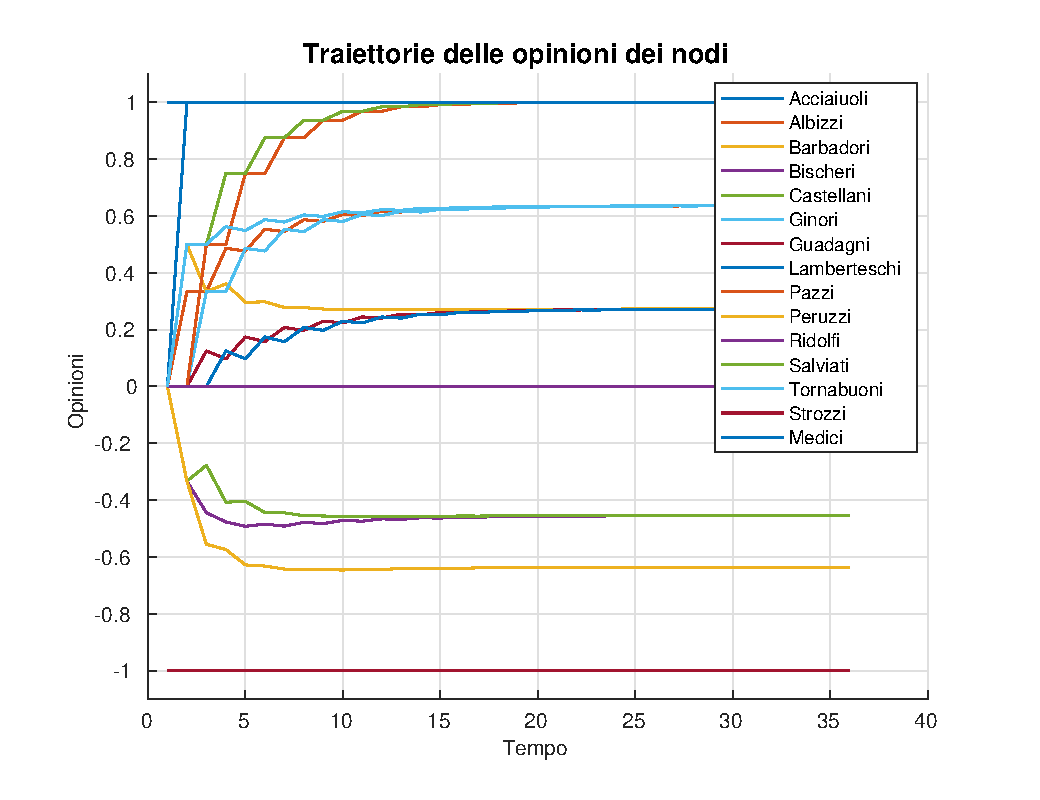
\includegraphics[scale=0.6]{traiettorie}%
\end{figure}

Il vettore di equilibrio $x(t)$ vale: 
\[x(t)=\begin{pmatrix}
    1.0000 \\
    0.6363 \\
    0.2727 \\
   -0.4546 \\
   -0.4546 \\	
    0.6362 \\
    0.2725 \\
    0.2726 \\
    1.0000 \\
   -0.6364 \\
         0 \\
    1.0000 \\
    0.6363 \\
   -1.0000 \\
    1.0000    
\end{pmatrix}\]
\item%3c
L'insieme dei nodi stubborn $S=\{Castellani, Guadagni, Medici, Strozzi\}$ è globalmente raggiungibile. Sia $D=diag(\omega_i)$ e \(P\) la matrice dei pesi normalizzata. 
\[P=D^{-1}W=\begin{bmatrix} 
0 & 0 & 0 & 0 & 0 & 0 & 0 & 0 & 0 & 0 & 0 & 0 & 0 & 0 & 1\\
0 & 0 & 0 & 0 & 0 & \frac{1}{3} & \frac{1}{3} & 0 & 0 & 0 & 0 & 0 & 0 & 0 & \frac{1}{3} \\
0 & 0 & 0 & 0 & \frac{1}{2} & 0 & 0 & 0 & 0 & 0 & 0 & 0 & 0 & 0 & \frac{1}{2}\\
0 & 0 & 0 & 0 & 0 & 0 & \frac{1}{3} & 0 & 0 & \frac{1}{3} & 0 & 0 & 0 & \frac{1}{3} & 0\\
0 & 0 & \frac{1}{3} & 0 & 0 & 0 & 0 & 0 & 0 & \frac{1}{3} & 0 & 0 & 0 & \frac{1}{3} & 0\\
0 & 1 & 0 & 0 & 0 & 0 & 0 & 0 & 0 & 0 & 0 & 0 & 0 & 0 & 0\\
0 & \frac{1}{4} & 0 & \frac{1}{4} & 0 & 0 & 0 & \frac{1}{4} & 0 & 0 & 0 & 0 & \frac{1}{4} & 0 & 0\\
0 & 0 & 0 & 0 & 0 & 0 & 1 & 0 & 0 & 0 & 0 & 0 & 0 & 0 & 0\\
0 & 0 & 0 & 0 & 0 & 0 & 0 & 0 & 0 & 0 & 0 & 1 & 0 & 0 & 0\\
0 & 0 & 0 & \frac{1}{3} & \frac{1}{3} & 0 & 0 & 0 & 0 & 0 & 0 & 0 & 0 & \frac{1}{3} & 0\\
0 & 0 & 0 & 0 & 0 & 0 & 0 & 0 & 0 & 0 & 0 & 0 & 0 & \frac{1}{2} & \frac{1}{2}\\
0 & 0 & 0 & 0 & 0 & 0 & 0 & 0 & \frac{1}{2} & 0 & 0 & 0 & 0 & 0 & \frac{1}{2}\\
0 & 0 & 0 & 0 & 0 & 0 & \frac{1}{2} & 0 & 0 & 0 & 0 & 0 & 0 & 0 & \frac{1}{2}\\
0 & 0 & 0 & \frac{1}{4} & \frac{1}{4} & 0 & 0 & 0 & 0 & 0 & \frac{1}{4} & \frac{1}{4} & 0 & 0 & 0\\
\frac{1}{6} & \frac{1}{6} & \frac{1}{6} & 0 & 0 & 0 & 0 & 0 & 0 & 0 & \frac{1}{6} & \frac{1}{6} & 0 & 0
\end{bmatrix}\]
 

Pertanto, il vettore di equilibrio della dinamica di averaging è dato dalla risoluzione del seguente sistema lineare
\begin{equation}
	\begin{cases}
		x_5 = x_7 = x_{14} = -1\\
		x_{15} = +1\\
		x_i = \sum\limits_{j} P_{ij}x_j, \ j=\{1,2,3,4,6,8,9,10,11,12,13\}
	\end{cases}
\end{equation}	

\begin{equation}
	\begin{cases}
		x_5 = x_7 = x_{14} = -1\\
		x_15 = +1\\
		x_1 = x_15\\		
		x_2 = \frac{1}{3}x_6 + \frac{1}{3}x_7 + \frac{1}{3}x_15\\
		x_3 = \frac{1}{2}x_5 + \frac{1}{3}x_15\\
		x_4 = \frac{1}{3}x_7 + \frac{1}{3}x_{10} + \frac{1}{3}x_{14}\\
		x_6 = x_2\\
		x_8 = x_7\\
		x_{9} = x_{12}\\
		x_{10} = \frac{1}{3}x_4 + \frac{1}{3}x_5 + \frac{1}{3}x_{14}\\		
		x_{11} = \frac{1}{2}x_15 + \frac{1}{3}x_{14}\\
		x_{12} = \frac{1}{2}x_15 + \frac{1}{2}x_{9}\\
		x_{13} = \frac{1}{2}x_7 + \frac{1}{2}x_15\\	
	\end{cases}
\end{equation}	

La soluzione del sistema è
\begin{equation}
x(t)=[1,0,0,-1,-1,0,-1,-1,1,-1,0,1,-1,0,1]'
\end{equation}
da cui si deduce che Acciaiuoli, Pazzi e Salviati avranno la stessa opinione dei Medici pari a $+1$ mentre Bischeri, Castellani, Guadagni, Lamberteschi, Peruzzi e Strozzi condivideranno l'opinione $-1$ ed i restanti Albizzi, Barbadori, Ginori, Ridolfi e Tornabuoni manterranno l'opinione iniziale pari a $0$.  

\item %3d 
Il vettore di centralità Page-Rank $z$ è la soluzione dell'equazione 
\begin{equation}
z = (1-\beta)P'z +\beta\nu
\end{equation} che equivale a calcolare il limite per $t\to\infty$ della dinamica di rete 
\begin{equation}
y(t+1) = (1-\beta)P'y(t) + \lambda
\end{equation}
dove $\lambda = \beta\nu$.
%\[\lim_{t \to \infty} y_i(t)= z\] 

Di seguito il codice Matlab utilizzato. 

\begin{lstlisting}
%y_new=Q'y_old+lambda
n = 15; 
beta = 0.15; 
nu = (1/n)*ones(n,1);       %entrata uniforme
Q = (1-beta)*P; 
lambda = beta*nu;

%inizializzazioni
cont_max = 60;       	%stima iterazioni necessarie
y_old = zeros(n,1); 
y_new = zeros(n,1);
Y_i = zeros(n,cont_max); 

eps = 1e-4;         %tolleranza
flag = 1;           %valuta se proseguire in base alla tolleranza
cont = 0; 

while(flag && cont < cont_max)
    cont = cont+1; 
    y_new = Q'*y_old + lambda;
    if(y_new - y_old <= epsilon)
        flag = 0; 
    else
        y_old = y_new; 
    end 
end
\end{lstlisting}

Il vettore di centralità ottenuto è il seguente.
\[z(t)=\begin{pmatrix}
0.0317\\ 
0.0819\\ 0.0519\\ 0.0713\\ 0.0714\\ 0.0332\\ 0.1033\\ 0.0319\\ 0.0367\\ 0.0699\\ 0.0513\\ 0.0630\\ 0.0537\\ 0.0920\\ 0.1535\\
\end{pmatrix}\]. 
\end{enumerate}

\end{document}